\documentclass{article}

\usepackage{graphicx}
\usepackage{multirow}
\usepackage{color}
\usepackage[citecolor=black,linkcolor=black,urlcolor=blue,colorlinks=true]{hyperref}
\title{Note: Neural Networks}
\author{Sun Zhao}

\begin{document}
\maketitle
\newpage

\section{Representation}
Brain makes human to learn and gain knowledge. So, what's the structure inside brain and how does brain learn? The answer is neural networks. In biology, neural networks inside our brains consist of billions of neurons, each of which can produce and transfer biological information to others and receive from others too. In machine learning field, neural networks are algorithms that mimic our brain's neural networks. Fig. \ref{neuron_model} shows a simple neuron having several inputs and one output. There are weights/parmeters on each edge between neurons to represent how strong the connection is. Each neuron collects all the weighted inputs, performs self-defined calculation and produces weighted output. We use an activation function to define the calculation performed on each neuron. Fig .\ref{logistic_neuron_unit} shows a logistic neuron consisting of a sigmoid activation function and an extra bias unit of $x_{0}$. Fig. \ref{neural_networks} shows a typical neural networks including input layer, hidden layer and output layer. Neurons between layer i and layer i +1 are pair-wise connected. Calculations performed on each neuron are shown in the bottom of Fig. \ref{neural_networks}.
\begin{figure}[ht]
  \centering
  % Requires \usepackage{graphicx}
  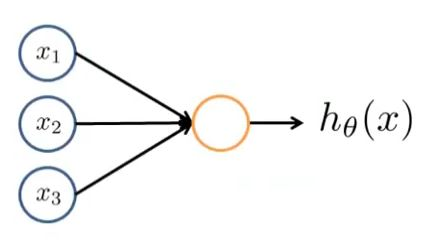
\includegraphics[width=3cm]{Figure1.jpg}\\
  \caption{Neuron Model}\label{neuron_model}
\end{figure}
\begin{figure}[ht]
  \centering
  % Requires \usepackage{graphicx}
  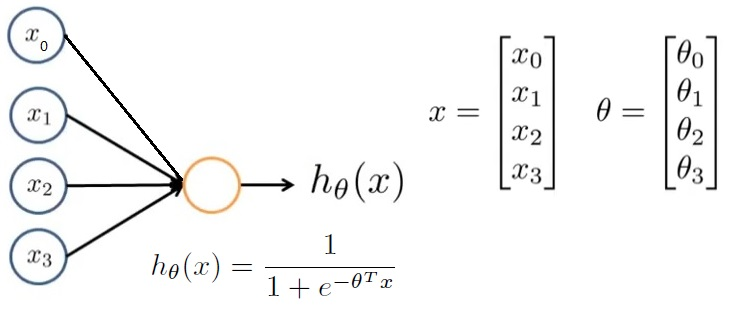
\includegraphics[width=5cm]{Figure2.jpg}\\
  \caption{Logistic Neuron Unit}\label{logistic_neuron_unit}
\end{figure}
\begin{figure}[ht]
  \centering
  % Requires \usepackage{graphicx}
  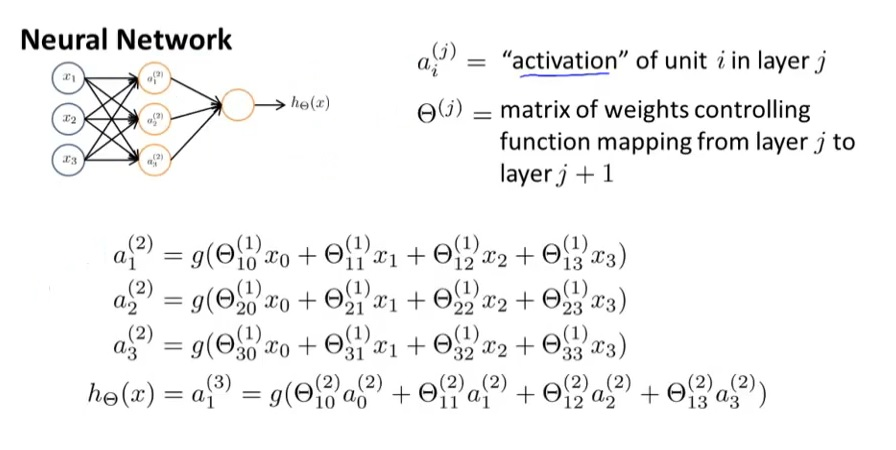
\includegraphics[width=9cm]{Figure3.jpg}\\
  \caption{Neural Networks}\label{neural_networks}
\end{figure}
\section{Motivation}
Let's see an classification problem shown in Fig. \ref{XOR_classification_problem}. Obviously, there does not exists a linear curve separating the two classes. However, a logic function of $x_{1}$ XOR $x_{2}$ classifies the two classes perfectly. Neural networks are good at these non-linear problems, and we can build a neural network to solve the XOR classification problem. Using the logistic neuron unit in Fig. \ref{logistic_neuron_unit}, we can first get three logic classifiers shown in Fig. \ref{logic_neurons}. To verify the correctness of these three logic classifiers, you may draw the truth table. Combining the three logic neurons, Fig. \ref{XOR_neural_networks} shows the final neural networks to solve the XOR classification problem with its truth table on the right.
\begin{figure}[ht]
  \centering
  % Requires \usepackage{graphicx}
  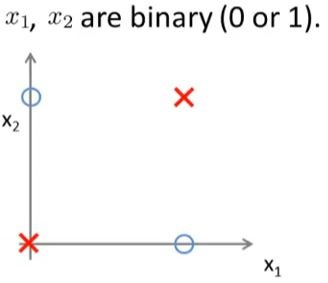
\includegraphics[width=3cm]{Figure4.jpg}\\
  \caption{Neuron Model}\label{XOR_classification_problem}
\end{figure}
\begin{figure}[ht]
  \centering
  % Requires \usepackage{graphicx}
  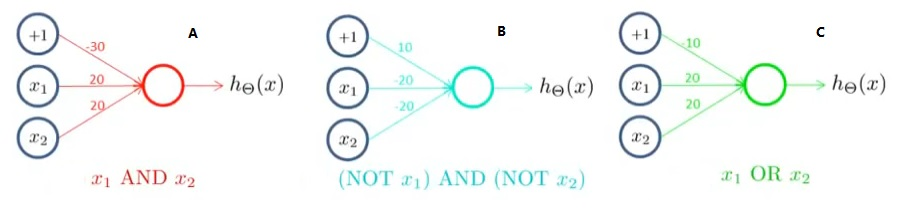
\includegraphics[width=10cm]{Figure5.jpg}\\
  \caption{Neuron Model}\label{logic_neurons}
\end{figure}
\begin{figure}[ht]
  \centering
  % Requires \usepackage{graphicx}
  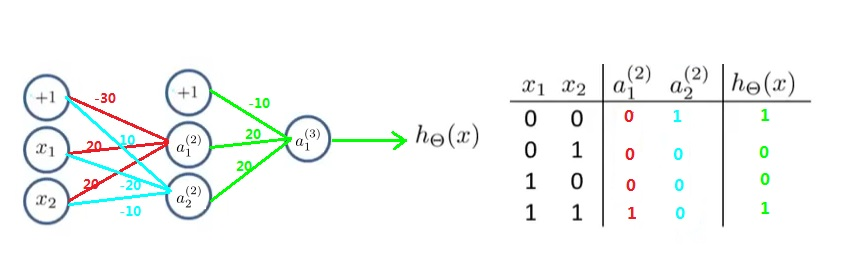
\includegraphics[width=10cm]{Figure6.jpg}\\
  \caption{Neuron Model}\label{XOR_neural_networks}
\end{figure}
\section{Cost Function}
Generally, neural networks outputs k hypothesis when solving a k classes classification problem. Using notations shown in Tab. \ref{neural_networks_cost_function_notation} and regularized logistic regression cost function, the neural networks' cost function is defined as (\ref{neural_networks_cost_function}).
\begin{table}[hb]
\begin{center}
\caption{}\label{neural_networks_cost_function_notation}
\begin{tabular}{l|l}
\hline
Notation & Meaning\\
\hline
L   & total No. of layers\\
$s_{l}$ & No. of units in layer l\\
K   & No. of output units \\
$(h_{\Theta}(x))_{i}$ & $i_{th}$ output hypothesis\\
\hline
\end{tabular}
\end{center}
\end{table}
\begin{equation}\label{neural_networks_cost_function}
J(\Theta) = -\frac{1}{m}\biggl[\sum_{i=1}^{m}\sum_{k=1}^{K} y_{k}^{(i)}log(h_{\Theta}(x^{(i)}))_{k} + (1 - y_{k}^{(i)})log(1 - (h_{\Theta}(x^{(i)}))_{k})\biggr] + \frac{\lambda}{2m}\sum_{l=1}^{L-1}\sum_{i=1}^{s_{l}}\sum_{j=1}^{s_{l+1}}(\Theta_{ji}^{(l)})^{2}
\end{equation}
The index of i starts from 1 instead of 0 is because the bias is always ignored to be regularized.

\section{Forward and Backward Propagation}
When implementing gradient descent algorithm, we need compute $J(\Theta)$ and the partial derivative terms of $\frac{\partial}{\partial \Theta_{ij}^{(l)}}$ for all i, j, and l. Forward and backward propagation are used to calculate the two terms. Fig. \ref{four_layer_neural_networks} shows a four-layer neural networks. Starting from the first layer and calculate output as input of previous layer iteratively, the final hypothesis will be the last output. Concretely, we can use following procedure to compute the hypothesis for Fig. \ref{four_layer_neural_networks}'s neural networks.

\begin{table}[hb]
\begin{center}
\begin{tabular}{rcl}
$a^{(1)}$ &= &x\\
$z^{(2)}$ &= &$\Theta^{(1)}a^{(1)}$\\
$a^{(2)}$ &= &$g(z^{(2)})$(add $a_{0}^{(2)}$)\\
$z^{(3)}$ &= &$\Theta^{(2)}a^{(2)}$\\
$a^{(3)}$ &= &$g(z^{(3)})$(add $a_{0}^{(3)}$)\\
$z^{(4)}$ &= &$\Theta^{(3)}a^{(3)}$\\
$a^{(4)}$ &= &$h_{\Theta}(x)=g(z^{(4)})$\\
\end{tabular}
\end{center}
\end{table}

\begin{figure}[ht]
  \centering
  % Requires \usepackage{graphicx}
  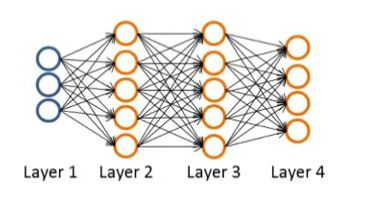
\includegraphics[width=5cm]{Figure7.jpg}\\
  \caption{Neuron Model}\label{four_layer_neural_networks}
\end{figure}
To calculate the derivative terms, we introduce a new notation of $\delta_{j}^{(l)}$ to represent the error of node j on layer l. For the output unit, it is obvious that $\delta_{j}^{(L)} = a_{j}^{(L)} - y_{j}^{(L)}$, and for layers which is prior to L, (\ref{delta_backward_propagation}) is used to iteratively calculate its value. The term $g'(z^{(l)})$ in (\ref{delta_backward_propagation}) can be extended to $a^{(l)}.*(1-a^{(l)})$.
\begin{equation}\label{delta_backward_propagation}
\delta^{(l)} = (\Theta^{(l)})^{T}\delta^{(l+1)}.*g'(z^{(l)})
\end{equation}
Algorithm 1 shows the back propagation process and output all layers' $\delta$ values with which we can define $\frac{\partial}{\partial \Theta_{ij}^{(l)}}$ as (\ref{partial_derivative_defination}). The prove of Algorithm 1 and (\ref{delta_backward_propagation}) is skipped, and I cannot figure it out myself. The partial derivative terms' calculation is quit obscure and different from that in logistic regression gradient descent process. I need refer other references to find more details.
\smallskip
\hrule
\smallskip
Algorithm 1: Back Propagation
\smallskip
\hrule
\smallskip
Training set$\{(x^{(1)}, y^{(1)}), (x^{(2)}, y^{(2)}), $\ldots$ , (x^{(m)}, y^{(m)})\}$\\
Set $\Delta_{ij}^{(l)}$ = 0 for all i, j, l\\
For i = 1 to m\\
\indent $a^{(1)} = x^{(i)}$\\
\indent Perform forward propagation to compute $a^{(l)}$ for l=2,3, $\ldots$, L\\
\indent Using $y^{(i)}$ to compute $\delta^{(L)} = a^{(L)} - y^{(i)}$\\
\indent Compute $\delta^{(L-1)}, \delta^{(L-2)}, \ldots, \delta^{(2)}$\\
\indent $\Delta_{ij}^{(l)} = \Delta_{ij}^{(l)} + a_{j}^{(l)}\delta_{i}^{(l+1)}$\\
\hrule
\medskip
\begin{equation}\label{partial_derivative_defination}
\frac{\partial}{\partial \Theta_{ij}^{(l)}}J(\Theta) = D_{ij}^{(l)} = \left\{ \begin{array}{ll}
\frac{1}{m}\delta_{ij}^{(l)} + \lambda \Theta_{ij}^{(l)} & \textrm{if j $\neq$ 0}\\
\frac{1}{m}\delta_{ij}^{(l)} & \textrm{if j = 0}\\
\end{array} \right.
\end{equation}

\section{Gradient Checking}
Since the back propagation algorithm is much complicated, the implementation of it needs a double checking for all the partial derivatives. We can use an derivative approximation shown in (\ref{approximate_derivative}) to write an Octave function to check whether gradApprox(approximation derivative) $\approx$ Dvec(output of back propagation). The last thing we need pay attention is to turn off the gradient checking after learning, otherwise, it will be very slow for predicting new values.
\begin{equation}\label{approximate_derivative}
\frac{d}{d\theta}J(\theta) = \frac{J(\theta + \epsilon) + J(\theta - \epsilon)}{2 \epsilon}
\end{equation}

\newpage
\smallskip
\hrule
\smallskip
Gradient Checking\\
\smallskip
\hrule
\smallskip
\noindent for i= 1:n\\
\indent thetaPlus = theta;\\
\indent thetaPlus(i) = thetaPlus(i) + EPSILON;\\
\indent thetaMinus = theta;\\
\indent thetaMinus(i) = thetaMinus(i) - EPSILON;\\
\indent gradApprox(i) = (J(thetaPlus) - J(thetaMinus)) / (2*EPSILON);\\
end;\\
\hrule
\medskip

\section{Random Initialization}
Recall that in logistic regression gradient descent, the initial parameters of $\Theta$ all is set to zero. However, if this initialization strategy is adopted on neural networks, no matter how many iterations have been processed, the parameters to the same neuron are all identical. Hence, we need a random initialization to break this symmetry. In Octave, \emph{rand(m, n)*(2*EPSILON) - EPLISON} can generate a random m$\times$n dimensional matrix with all element between -EPSLION and +EPSLION.

\section{Summary}
Neural networks mimics the structure of human brain, and shows power on non-linear classification problem. We use forward and backward propagation to calculate $J(\Theta)$ and $\frac{\partial}{\partial \Theta_{ij}^{(l)}}$ separately. When implementing back propagation algorithm, it is suggested to use a gradient checking and random initialization. At last, the succeed of autonomous driving based on neural networks really shows the power of machine learning.
\end{document}
